\documentclass[11pt]{article}
\usepackage[margin=1in]{geometry}
\usepackage{amsmath,amssymb}
\usepackage{tikz}
\usetikzlibrary{arrows.meta}

\title{Proof Summary: NP-Hardness of the Ordering Recovery Problem}
\date{}

\begin{document}
\maketitle

\noindent This document gives an informal overview of the proof that the Ordering Recovery Problem (ORP) is NP-hard, via a many-one reduction from the Minimum Feedback Arc Set in Tournaments (FAST) problem. The full rigorous proof is in the companion document.

\section*{The two problems}

\textbf{FAST.} Given a tournament $T$ (a complete directed graph on $N$ vertices) and an integer $k$: is there a linear ordering of the vertices with at most $k$ ``backward'' arcs?

\textbf{ORP.} Given $N$ events with noisy observed timestamps and a threshold $K$: is there a permutation $\hat{\pi}$ whose expected Kendall tau distance to the unknown true ordering is at most $K$?

\section*{Key idea}

Every edge of the tournament gets encoded as a pair of events whose relative ordering is uncertain. The noise distributions are rigged so that:
\begin{itemize}
\item each event pair can only occupy two adjacent time slots (a ``block''),
\item the posterior probability favours the ordering that matches the arc direction,
\item getting a pair wrong costs the same amount ($1/2$) regardless of which pair it is.
\end{itemize}
This makes the ORP cost proportional to the number of backward arcs, i.e., to $\mathrm{fas}(T, \pi')$.

\section*{Proof outline in five steps}

\subsection*{Step 1: Pairwise decomposition (Lemmas 1--2)}

The expected Kendall tau distance decomposes as a sum over all pairs of events. For each pair $(i, j)$, the contribution depends on whether $\hat{\pi}$ agrees or disagrees with the \emph{most-likely ordering} (the ordering with higher posterior probability). Disagreeing costs $|2p_{ij} - 1|$ more than agreeing.

\subsection*{Step 2: Construct the ORP instance}

Given a tournament $T$ on $N$ vertices with $M = \binom{N}{2}$ edges:

\begin{center}
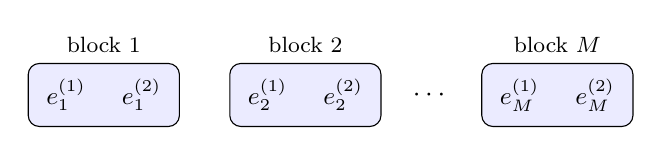
\begin{tikzpicture}[>=Stealth, scale=0.8]
  \draw[rounded corners, fill=blue!8] (0,0) rectangle (2.4,1);
  \node[font=\footnotesize] at (1.2,1.3) {block 1};
  \node[font=\small] at (0.6,0.5) {$e_1^{(1)}$};
  \node[font=\small] at (1.8,0.5) {$e_1^{(2)}$};
  
  \draw[rounded corners, fill=blue!8] (3.2,0) rectangle (5.6,1);
  \node[font=\footnotesize] at (4.4,1.3) {block 2};
  \node[font=\small] at (3.8,0.5) {$e_2^{(1)}$};
  \node[font=\small] at (5.0,0.5) {$e_2^{(2)}$};
  
  \node at (6.4,0.5) {$\cdots$};
  
  \draw[rounded corners, fill=blue!8] (7.2,0) rectangle (9.6,1);
  \node[font=\footnotesize] at (8.4,1.3) {block $M$};
  \node[font=\small] at (7.8,0.5) {$e_M^{(1)}$};
  \node[font=\small] at (9.0,0.5) {$e_M^{(2)}$};
\end{tikzpicture}
\end{center}

Each edge $\{i_r, j_r\}$ of the tournament becomes a block of two events in adjacent time slots. The noise distributions have finite support, which forces each event to stay in its own block. This is the key piece of cleverness: the noise is engineered so that the \emph{true} timestamps (not just the observed ones) are confined to the block.

\subsection*{Step 3: Compute posteriors}

Using Bayes' rule, the posterior probability that $e_r^{(1)}$ precedes $e_r^{(2)}$ is $3/4$ or $1/4$ depending on the arc direction. Writing $p_r = P(e_r^{(1)} \text{ truly precedes } e_r^{(2)} \mid \hat{t})$ for this posterior, in both cases:
\begin{itemize}
\item the most-likely ordering matches the arc direction in $T$,
\item the disagreement weight is $|2p_r - 1| = 1/2$ for every pair.
\end{itemize}

\subsection*{Step 4: Connect ORP cost to feedback arc set}

Because inter-block orderings are deterministic (events in earlier blocks always precede events in later blocks) and intra-block decisions are independent, the expected Kendall tau distance for a ``lifted'' permutation (one that respects block order) is:
\[
\mathbb{E}[d_{\mathrm{KT}}(\hat{\pi}, \sigma) \mid \hat{t}] = \frac{1}{2} \cdot \mathrm{fas}(T, \pi') + \frac{M}{4},
\]
where $\pi'$ is the vertex ordering that determines each block's internal order. Moreover, any arbitrary permutation can be improved to a lifted one (with cost at most as large), because fixing inter-block disagreements can only reduce the cost.

\subsection*{Step 5: Complete the reduction}

Set the ORP threshold to $K = k/2 + M/4$. Then:

\begin{itemize}
\item ($\Rightarrow$) If $\mathrm{fas}(T, \pi') \le k$, lifting $\pi'$ gives a permutation with cost $\le K$.
\item ($\Leftarrow$) If some permutation has cost $\le K$, improving it to a lifted one gives a vertex ordering with $\mathrm{fas} \le k$.
\end{itemize}

The construction runs in polynomial time ($2M = N(N-1)$ events, $O(1)$ parameters each). Since FAST is NP-complete, ORP is NP-hard. $\square$

\end{document}
